\documentclass{article}
\usepackage{amsmath, amssymb, amsfonts, amsthm}
\usepackage{url, graphicx}
\numberwithin{equation}{section}
\linespread{1.2}
\title{An Introduction to Artificial Neural Networks}
\author{To be filled}
\date{24-Oct-2020}
\begin{document}
\maketitle
\section{Introduction}\label{s1}
Many inventions were inspired by observing Nature's creations. The burrs of
burdock clinging to his dress inspired George de Mestral to think of an
interlocking system of tiny threads leading him to develop Velcro. The ability
of bats to navigate in absence of light inspired people to build SONAR to
sense obstacles in deep water where light does not reach. It is, therefore,
not surprising that the human brain were the most obvious object to mimic
when people started thinking about artificial intelligence in the 1930s and 40s.
In this article, we will trace the development of artificial neural networks
since their inception in the first half of the twentieth century till today.
It is customary to begin a discussion of artificial neural networks by first
taking a glimpse of their immensely more powerful natural cousins.

The human brain has a very large number, of the order of $10^{11}$, specialized
cells called neurons. They are also some of the largest cells in the human
body. The cell body of the neuron is called the \emph{soma}. It has many 
hair-like extensions called the \emph{dendrites} and a single, long, tail-like
extension called the \emph{axon}. Figure \ref{f1} shows a schematic diagram of
a neuron.

The axon of one neuron is connected to the dendrites of other neurons through
a connection called the \emph{synapse}. Neurons are electrically conducting
cells. The inputs to a neuron arrive through their dendrites and soma and the 
output is made available by the axon. These features were first abstracted
into an artificial neuron by McCulloch and Pitts in their landmark paper 
\cite{mcculloch1943logical} of 1943 marking the beginning of the subject of
artificial neural networks. Their `neuron' had $m$ `dendrites' providing 
inputs $x_1, \ldots, x_m$. The dendrites were either in an `off' state or an
`on' state. If a sufficient number of `dendrites' were in an `on' state then 
they triggerd the `axon' to be in an `on' state. Mathematically, one can 
express this neuron as
\begin{equation}\label{s1e1}
y = \varphi\left(\sum_{j=1}^m w_j x_j\right),
\end{equation}
where $w_1, \ldots, w_m$ are the `weights' associated with the $m$ inputs and
the function $\varphi$ mapped its domain to $\{0, 1\}$. As the `neurons' took
boolean inputs and produces a boolean output they were a way to evaluate
logical expressions. McCulloch and Pitts proved that one could evaluate an
arbitrary expression of propositional logic with their `neurons' under certain
conditions \cite{mcculloch1943logical}. They also showed that a network of
`neurons' are capable of universal computation \cite{bishop1994neural}. The
relaxation of the condition that the inputs and outputs can take only boolean
values was the next step in the development of artificial neurons. We cover it
in the next section.
\begin{figure}[!ht]
\centering
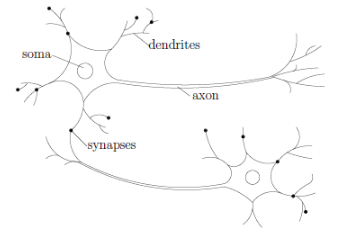
\includegraphics[scale=0.5]{neuron}
\caption{A neuron}
\label{f1}
\end{figure}

We mentioned weights $w_1, \ldots, w_m$ but did not reveal their role. Every
boolean expression requires a different neuron. Two neurons for different
boolean expressions with the same number of inputs differ in the weights 
attached to each input. `Training' an artificial neuron to decide a boolean
expression is the selection of weights so that the output is what we want.

\section{The Perceptron}\label{s2}
The American psychologist Frank Rosenblatt modified the McCulloch-Pitts neuron
allowing it take arbitrary inputs instead of boolean 
\cite{rosenblatt1958perceptron}. The function $\varphi$ in equation \eqref{s1e1}
was chosen to take the form of a step function
\begin{equation}\label{s2e1}
\theta(x) = \begin{cases}
0 \text{ if } x < 0 \\
1 \text{ if } x \ge 0.
\end{cases}
\end{equation}
The inputs $x_1, \ldots, x_m$ were augmented with a `bias' input $x_0$ which
was always $1$. The `weights' $w_1, \ldots, w_m$ were chosen in such a manner
that for most inputs $x_1, \ldots, x_m$, the perceptron produces the correct
output $y$. The algorithm to select the weights was also inspired by the way
biological neurons aid in human learning. The Canadian psychologist Donald Hebb
proposed \cite{hebb1949organization} that `neurons that fire together, wire
together', meaning that the connection between neurons grows if they are both
involved in a learning process. This suggested Rosenblatt that he should 
adjust the weights of the inputs based on the whether a given set of weights
produces correct output or not. Conversely, the weights are not adjusted if
they produce a correct output. We will demonstrate the perceptron learning
algorithm on the famous `iris' data set. The first step in data analysis is
always examining the data, which we do in the code below.
\begin{verbatim}
import numpy as np
import pandas as pd
import seaborn as sns
from sklearn import datasets
from sklearn.model_selection import train_test_split

df = sns.load_dataset("iris")
plot = sns.pairplot(df, hue="species")
plot.savefig('iris_pairplot.png')
\end{verbatim}

The pair plot of the four attributes of the data is
\begin{figure}[!ht]
\centering
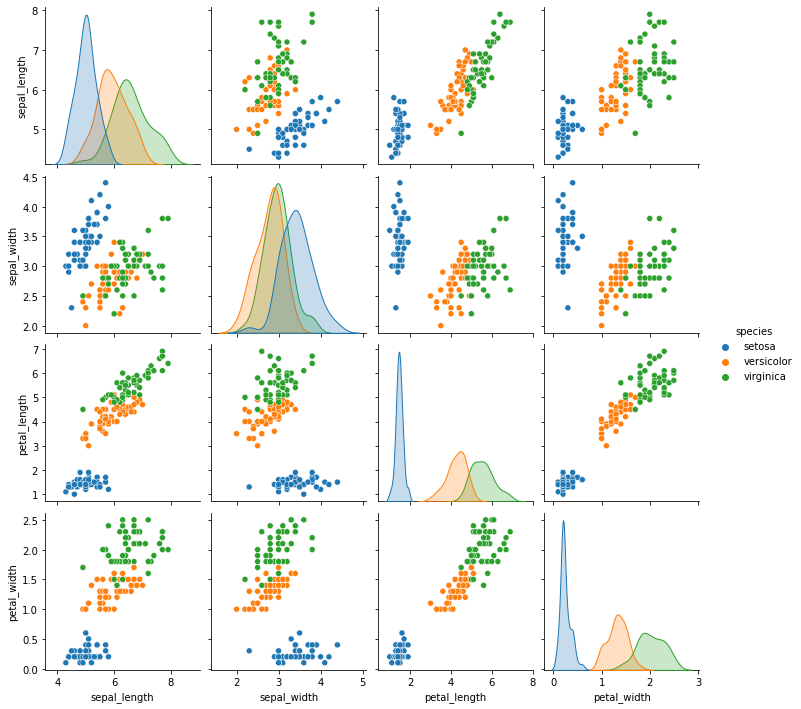
\includegraphics[scale=0.4]{iris}
\caption{Attributes of the iris dataset}
\label{f2}
\end{figure}

The pair plot in figure \ref{f2} suggests that petal width and petal length
are the best choice of attributes to tell the Setosa flowers from the other
two varieties. We add another attribute to the data set which takes a value
$1$ if the flower is Setosa and $-1$ if it is not. We then split the entire
data set into training and test data.

\begin{verbatim}
df['Class'] = np.where(df['species'] == 'setosa', 1, -1)
X_train, X_test, y_train, y_test = 
	train_test_split(df[['petal_length', 'petal_width']], \
                     df['Class'], \
                     test_size=1/3, \
                     random_state = 15081947)
\end{verbatim}

The next code listing has the core of the perceptron learning algorithm. We 
initialize weights to a small positive value. They are updated if for an 
observation the algorithm misclassifies it.
\begin{verbatim}
w = np.array([0.1, 0.1, 0.1]) 

def adjust_weights(X, y):
  global w
  z = X[0]*w[0] + X[1]*w[1] + w[2]
  if z > 0:
    y_hat = 1
  else:
    y_hat = -1
    
  w[0] += (y - y_hat) * X[0]
  w[1] += (y - y_hat) * X[1]
  w[2] += 1
\end{verbatim}

After running the algorithm on all observations in the training data set
we check its performance first on the training data set and then on the
test data set.
\begin{verbatim}
trn = pd.concat([X_train, y_train], axis=1)
tst = pd.concat([X_test, y_test], axis=1)
ignore = 
  trn.apply(lambda r: adjust_weights(r[['petal_length', 'petal_width']], \
            r['Class']), axis=1)

def classify(r):
  global w
  x = r[0]*w[0] + r[1]*w[1] + w[2]
  if x > 0:
    return 1
  else:
    return -1

trn_predict = trn.apply(lambda r: classify(r), axis=1)
tst_predict = tst.apply(lambda r: classify(r), axis=1)
\end{verbatim}

A cross-tabulation of the predicted and actual class shows that only $2$
out of $100$ training samples were misclassified. Repeating this step on
the test data shows that $3$ out of $50$ samples were misclassified. This 
error rate is not bad given the very simple algorithm we have used. We 
used this code to illustrate the essentials of the perceptron learning 
algorithm. A serious exercise in classification should use the perceptron
provided in the package \texttt{sklearn}. The code 
listing below shows that code.
\begin{verbatim}
from sklearn.linear_model import Perceptron

perceptron = Perceptron(random_state=26011950)
perceptron.fit(X_train, y_train)
y_pred = perceptron.predict(X_test)
\end{verbatim}
A cross-tabulation of the actual and the predicted class shows $100\%$
accuracy.

Equation \eqref{s2e1} is one choice of $\varphi$, the \emph{activation
function}. There are many others, some of which are shown in figure
\ref{f3}.
\begin{figure}[!ht]
\centering
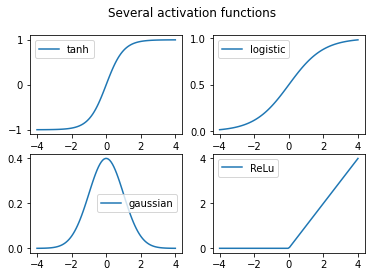
\includegraphics[scale=0.8]{activation}
\caption{Activation functions}
\label{f3}
\end{figure}

The perceptron was a sensation when it was first developed. It was 
implemented as hardware. However, it was soon discovered that it was
incapable of solving simple problems like the famous XOR problem. If
an output is an exclusive OR of its input then one cannot train a 
perceptron to evaluate it. In fact, it was soon shown that a perceptron 
functions best when there is a linear boundary separating the various
classes of inputs. Several problems do not have such a boundary and
therefore they are outside the purview of a perceptron.

\section{Multi-level Perceptrons}\label{s3}
Some limitations of a single perceptron can be overcome by building a
network of perceptrons. The term `multi-level perceptron' is network of
perceptrons with one layer taking inputs, another one producing the output
and one or more intermediate layers. It does not mean a perceptron with
multiple layers. It is a stack of perceptrons. Although the idea of a 
network of neurons was explored since the times of McCulloch and Pitts model
there is no algorithm to train the networks. In this section we will 
describe feed-forward multi-level perceptrons. The adjective `feed-forward'
means that the output of a neuron is not fed as an input to itself or
another neuron of a previous layer.

We summarize the behavior of a single perceptron in the following
equations \cite{bishop1994neural}.
\begin{eqnarray}
\sum_{i=0}^d w_i x_i &=& a \label{s3e1} \\
g(a) &=& z \label{s3e2},
\end{eqnarray}
where the input $x_0$ is always $1$, there are $d$ other inputs $x_1, 
\ldots, x_d$ and $g$ is a suitable activation function. We consider a
multi-layer perceptron with just a single hidden layer with a topology
shown in figure \ref{f4}.
\begin{figure}[!ht]
\centering
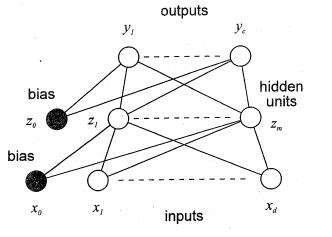
\includegraphics[scale=0.8]{mlp}
\caption{Multi-layer perceptron (from ref. \cite{bishop1994neural})}
\label{f4}
\end{figure}
There are $d + 1$ inputs and $m$ outputs in the first layer. The $m$ 
outputs are the inputs to the $m$ neurons in the second layer. The output
of every neuron in the first layer is fed as an input to the second layer.
Therefore there are $(d + 1) \times m$ weights, denoted by $w_{ij}$ with
$i$ ranging from $0$ to $d$ and $j$ ranging from $1$ to $m$. Using the 
notations of equations \eqref{s3e1} and \eqref{s3e2}, we can write
\begin{equation}\label{s3e3}
z_j = g\left(\sum_{i=0}^d w_{ji}x_i\right).
\end{equation}

\bibliographystyle{plain}
\bibliography{nn}
\end{document}
